%% abtex2-modelo-artigo.tex, v-1.9.5 laurocesar
%% Copyright 2012-2015 by abnTeX2 group at http://www.abntex.net.br/ 
%%
%% This work may be distributed and/or modified under the
%% conditions of the LaTeX Project Public License, either version 1.3
%% of this license or (at your option) any later version.
%% The latest version of this license is in
%%   http://www.latex-project.org/lppl.txt
%% and version 1.3 or later is part of all distributions of LaTeX
%% version 2005/12/01 or later.
%%
%% This work has the LPPL maintenance status `maintained'.
%% 
%% The Current Maintainer of this work is the abnTeX2 team, led
%% by Lauro César Araujo. Further information are available on 
%% http://www.abntex.net.br/
%%
%% This work consists of the files abntex2-modelo-artigo.tex and
%% abntex2-modelo-references.bib
%%

% ------------------------------------------------------------------------
% ------------------------------------------------------------------------
% abnTeX2: Modelo de Artigo Acadêmico em conformidade com
% ABNT NBR 6022:2003: Informação e documentação - Artigo em publicação 
% periódica científica impressa - Apresentação
% ------------------------------------------------------------------------
% ------------------------------------------------------------------------

\documentclass[
	% -- opções da classe memoir --
	article,			% indica que é um artigo acadêmico
	12pt,				% tamanho da fonte
	twoside,			% para impressão apenas no verso. Oposto a twoside
	a4paper,			% tamanho do papel. 
	% -- opções da classe abntex2 --
	%chapter=TITLE,		% títulos de capítulos convertidos em letras maiúsculas
	%section=TITLE,		% títulos de seções convertidos em letras maiúsculas
	%subsection=TITLE,	% títulos de subseções convertidos em letras maiúsculas
	%subsubsection=TITLE % títulos de subsubseções convertidos em letras maiúsculas
	% -- opções do pacote babel --
	english,			% idioma adicional para hifenização
	brazil,				% o último idioma é o principal do documento
	sumario=tradicional
	]{abntex2-modelo-notas-de-aula}


% ---
% PACOTES
% ---

% ---
% Pacotes fundamentais 
% ---
\usepackage{lmodern}			% Usa a fonte Latin Modern
\usepackage[T1]{fontenc}		% Selecao de codigos de fonte.
\usepackage[utf8]{inputenc}		% Codificacao do documento (conversão automática dos acentos)

\usepackage{amsmath}
\usepackage{siunitx}
\sisetup{detect-all}
\sisetup{round-mode=places,round-precision=2}
\DeclareSIUnit \VA {VA} %apparent power

% ---
		
% ---
% Pacotes adicionais, usados apenas no âmbito do Modelo Canônico do abnteX2
% ---
\usepackage{lipsum}				% para geração de dummy text
% ---
		
% ---
% Pacotes de citações
% ---
\usepackage[brazilian,hyperpageref]{backref}	 % Paginas com as citações na bibl
\usepackage[alf]{abntex2cite}	% Citações padrão ABNT
% ---

%Numeração dos floats por capítulo
\counterwithin{figure}{section} 
\counterwithin{table}{section}
\counterwithin{equation}{section}



% ---
% Configurações do pacote backref
% Usado sem a opção hyperpageref de backref
\renewcommand{\backrefpagesname}{Citado na(s) página(s):~}
% Texto padrão antes do número das páginas
\renewcommand{\backref}{}
% Define os textos da citação
\renewcommand*{\backrefalt}[4]{
	\ifcase #1 %
	Nenhuma citação no texto.%
	\or
	Citado na página #2.%
	\else
	Citado #1 vezes nas páginas #2.%
	\fi}%
% ---


% ---
% Informações de dados para CAPA e FOLHA DE ROSTO
% ---
\centro{Centro Tecnológico}
\departamento{Departamento de Engenharia Elétrica e Eletrônica}
\local{Florianópolis}
\data{\today}

\autor{Prof. Adriano \textsc{Ruseler}, M. Eng.}

\tipotrabalho{Notas de Aula}
\disciplina{Eletrônica de Potência I}
\codigo{EEL 7074} % Código da disciplina
\semestre{2015/2}
\aula{Aula 01}
\titulo{Modelo Canônico de Notas de Aula com \abnTeX}

\preambulo{Modelo canônico de notas de aula em conformidade
	com as normas ABNT apresentado à comunidade de usuários \LaTeX.}



% ---
% Configurações de aparência do PDF final

% alterando o aspecto da cor azul
\definecolor{blue}{RGB}{41,5,195}

% informações do PDF
\makeatletter
\hypersetup{
     	%pagebackref=true,
		pdftitle={\@title}, 
		pdfauthor={\@author},
    	pdfsubject={Modelo de Notas de Aulas com abnTeX2},
	    pdfcreator={LaTeX with abnTeX2},
		pdfkeywords={abnt}{latex}{abntex}{abntex2}{notas de aula}, 
		colorlinks=true,       		% false: boxed links; true: colored links
    	linkcolor=black,          	% color of internal links
    	citecolor=black,        		% color of links to bibliography
    	filecolor=black,      		% color of file links
		urlcolor=black,
		bookmarksdepth=4
}
\makeatother
% --- 

% ---
% compila o indice
% ---
\makeindex
% ---

% ---
% Altera as margens padrões
% ---
\setlrmarginsandblock{3cm}{3cm}{*}
\setulmarginsandblock{3cm}{3cm}{*}
\checkandfixthelayout
% ---


% --- 
% Espaçamentos entre linhas e parágrafos 
% --- 

% O tamanho do parágrafo é dado por:
\setlength{\parindent}{1.3cm}

% Controle do espaçamento entre um parágrafo e outro:
\setlength{\parskip}{0.2cm}  % tente também \onelineskip

% Espaçamento simples
\SingleSpacing

% ----
% Início do documento
% ----
\begin{document}

% Seleciona o idioma do documento (conforme pacotes do babel)
%\selectlanguage{english}
\selectlanguage{brazil}

% Retira espaço extra obsoleto entre as frases.
\frenchspacing 


\imprimircapaUFSC 

% ]  				% FIM DE ARTIGO EM DUAS COLUNAS
% ---


% ---
% inserir o sumario
% ---
\pdfbookmark[0]{\contentsname}{toc}
\tableofcontents*
\cleardoublepage
% ---

% ----------------------------------------------------------
% ELEMENTOS TEXTUAIS
% ----------------------------------------------------------
\textual
\pagestyle{notasUFSC}




% ----------------------------------------------------------
% Introdução
% ----------------------------------------------------------
\section*{Introdução}
\addcontentsline{toc}{section}{Introdução}

Este documento e seu código-fonte são exemplos de referência de uso da classe
\textsf{abntex2} e do pacote \textsf{abntex2cite}. O documento exemplifica a
elaboração de publicação periódica científica impressa produzida conforme a ABNT
NBR 6022:2003 \emph{Informação e documentação - Artigo em publicação periódica
científica impressa - Apresentação}.

A expressão ``Modelo canônico'' é utilizada para indicar que \abnTeX\ não é
modelo específico de nenhuma universidade ou instituição, mas que implementa tão
somente os requisitos das normas da ABNT. Uma lista completa das normas
observadas pelo \abnTeX\ é apresentada em \citeonline{abntex2classe}.

Sinta-se convidado a participar do projeto \abnTeX! Acesse o site do projeto em
\url{http://www.abntex.net.br/}. Também fique livre para conhecer,
estudar, alterar e redistribuir o trabalho do \abnTeX, desde que os arquivos
modificados tenham seus nomes alterados e que os créditos sejam dados aos
autores originais, nos termos da ``The \LaTeX\ Project Public
License''\footnote{\url{http://www.latex-project.org/lppl.txt}}.

Encorajamos que sejam realizadas customizações específicas deste documento.
Porém, recomendamos que ao invés de se alterar diretamente os arquivos do
\abnTeX, distribua-se arquivos com as respectivas customizações. Isso permite
que futuras versões do \abnTeX~não se tornem automaticamente incompatíveis com
as customizações promovidas. Consulte \citeonline{abntex2-wiki-como-customizar}
par mais informações.

Este exemplo deve ser utilizado como complemento do manual da classe
\textsf{abntex2} \cite{abntex2classe}, dos manuais do pacote
\textsf{abntex2cite} \cite{abntex2cite,abntex2cite-alf} e do manual da classe
\textsf{memoir} \cite{memoir}. Consulte o \citeonline{abntex2modelo} para obter
exemplos e informações adicionais de uso de \abnTeX\ e de \LaTeX.

% ----------------------------------------------------------
% Seção de explicações
% ----------------------------------------------------------
\newpage
\section{Exemplos de comandos}


\subsection{Exemplo de equação}


Para a obtenção da corrente de carga é recomendável o emprego da Série de Fourier. Decompondo-se a tensão obtém-se a expressão \eqref{eq:2.77}.

\begin{equation}\label{eq:2.77}
	{v_L}(\omega t) = \sqrt 2 \,{V_2}\,\left[ {\frac{2}{\pi } - \frac{4}{{3\pi }}\,\cos \,(2\omega t) - \frac{4}{{15\pi }}\,\cos \,(4\omega t) - \, \ldots } \right]
\end{equation}

\subsection{Exemplo de tabela}


Table \ref{tab:inversormotorstep} shows the dc voltage distribution between each bus capacitor for different load conditions. As the load increases the system becomes more balanced  due to increased of real power processed and decrease of reactive power exchanged.


\begin{table}[!h]
	\caption{Bus capacitor voltage and inverter output current at no load (\#0), one load step (\#1), two load step (\#2) and  three load step (\#3) conditions.}
	\label{tab:inversormotorstep}
	\centering	
	\resizebox{\linewidth}{!}{%
		\begin{tabular}{r|r|r|r|r|r|r|r|r|r} \toprule
			&\multicolumn{3}{c|}{\textbf{Phase A}}&\multicolumn{3}{c|}{\textbf{Phase B}}&\multicolumn{3}{c}{\textbf{Phase C}}\\\hline	
			&$W_{a1}$&$W_{a2}$&$W_{a3}$&$W_{b1}$&$W_{b2}$&$W_{b3}$&$W_{c1}$&$W_{c2}$&$W_{c3}$\\\hline	
			$V_{\text{RMS\#0}} [\SI{}{\V}]$ & $\num{377.47}$ & $\num{395.33}$ & $\num{417.42}$ & $\num{378.45}$ & $\num{394.80}$ & $\num{416.93}$ & $\num{419.27}$ & $\num{395.06}$ & $\num{375.74}$\\\hline
			$I_{\text{RMS\#0}} [\SI{}{\A}]$ & $\num{2.1838}$ & $\num{2.2999}$ & $\num{3.5054}$ & $\num{2.1238}$ & $\num{2.4817}$ & $\num{3.4562}$ & $\num{3.5370}$ & $\num{2.3312}$ & $\num{2.1689}$\\\hline
			$V_{\text{RMS\#1}} [\SI{}{\V}]$ & $\num{393.00}$ & $\num{396.58}$ & $\num{413.86}$ & $\num{392.65}$ & $\num{398.69}$ & $\num{412.04}$ & $\num{413.92}$ & $\num{395.06}$ & $\num{375.74}$\\\hline
			$I_{\text{RMS\#1}} [\SI{}{\A}]$ & $\num{2.4742}$ & $\num{2.5153}$ & $\num{3.4450}$ & $\num{2.4563}$ & $\num{2.4768}$ & $\num{3.4246}$ & $\num{3.4667}$ & $\num{2.4784}$ & $\num{2.4238}$\\\hline
			$V_{\text{RMS\#2}} [\SI{}{\V}]$ & $\num{392.21}$ & $\num{394.49}$ & $\num{408.76}$ & $\num{392.63}$ & $\num{397.45}$ & $\num{405.32}$ & $\num{408.52}$ & $\num{398.12}$ & $\num{389.40}$\\\hline
			$I_{\text{RMS\#2}} [\SI{}{\A}]$ & $\num{2.6773}$ & $\num{2.6704}$ & $\num{3.7173}$ & $\num{2.6641}$ & $\num{2.6998}$ & $\num{3.5942}$ & $\num{3.6715}$ & $\num{2.6967}$ & $\num{2.6158}$\\\hline
			$V_{\text{RMS\#3}} [\SI{}{\V}]$ & $\num{389.67}$ & $\num{391.57}$ & $\num{401.79}$ & $\num{394.47}$ & $\num{398.27}$ & $\num{412.04}$ & $\num{401.66}$ & $\num{394.99}$ & $\num{386.27}$\\\hline
			$I_{\text{RMS\#3}} [\SI{}{\A}]$ & $\num{3.0143}$ & $\num{2.9992}$ & $\num{3.9555}$ & $\num{3.0152}$ & $\num{3.7978}$ & $\num{3.4246}$ & $\num{3.8671}$ & $\num{3.0002}$ & $\num{2.8989}$\\\hline
			\bottomrule
		\end{tabular}
	}
\end{table}

\subsection{Inserindo código fonte}

\begin{lstlisting}[caption={Leitura dos dados simulados e conversão para estados topológicos.},label={lst:leituradadossim}]
% Pré definições iniciais
nsub=3;  % Numero de Sunmódulos
nbits=2*nsub; % Numero de bits necessários para representar os estados
nlevels=2*nsub+1; % Numero total de níveis

% Leitura dos pontos gerados por simulação
time=data(1,:)'; % extrai vetor de tempo
PWM=logical(data(2:end,:))'; % Conversão dos pulsos PWM para estados lógicos

% Cria vetor de string binário com os estados correspondentes
binstates=num2str([PWM(:,1) PWM(:,3) PWM(:,5) PWM(:,7) PWM(:,9) PWM(:,11)]);
state=fi(bin2dec(binstates),0,nbits,0); % Objeto numérico de ponto-fixo
\end{lstlisting}

\subsection{Figuras}



\begin{figure}[!h]
	\centering
	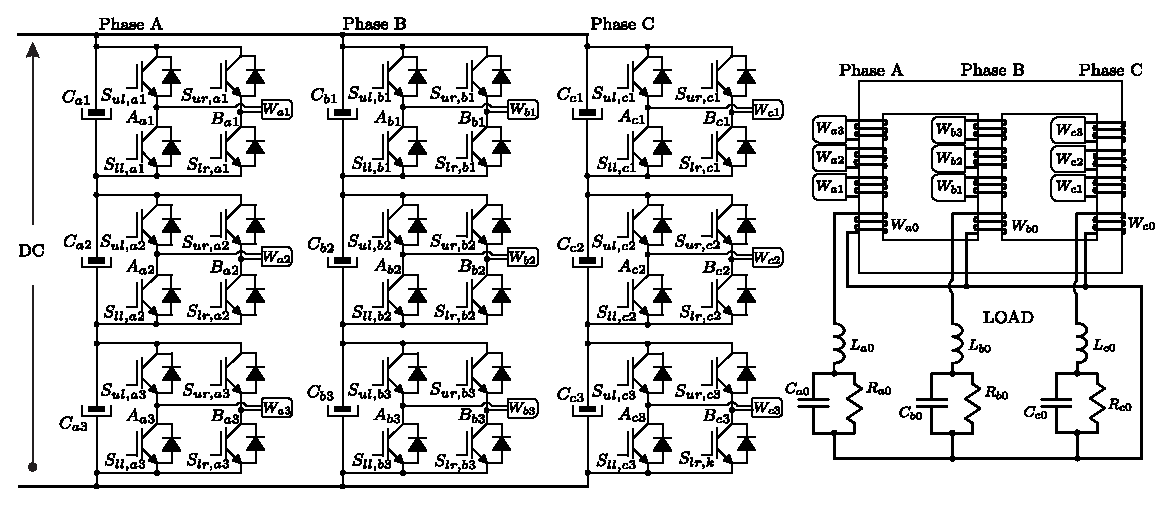
\includegraphics[width=1\linewidth]{figs/InversorTransformador}
	\caption{Conexão utilizada ao se empregar um transformador.}
	\label{fig:InversorTransformador}
\end{figure}


\subsection{Apresentando aquisições}


\begin{figure}[!h]
	\centering
	\begin{minipage}[t]{0.45\textwidth}	\centering
		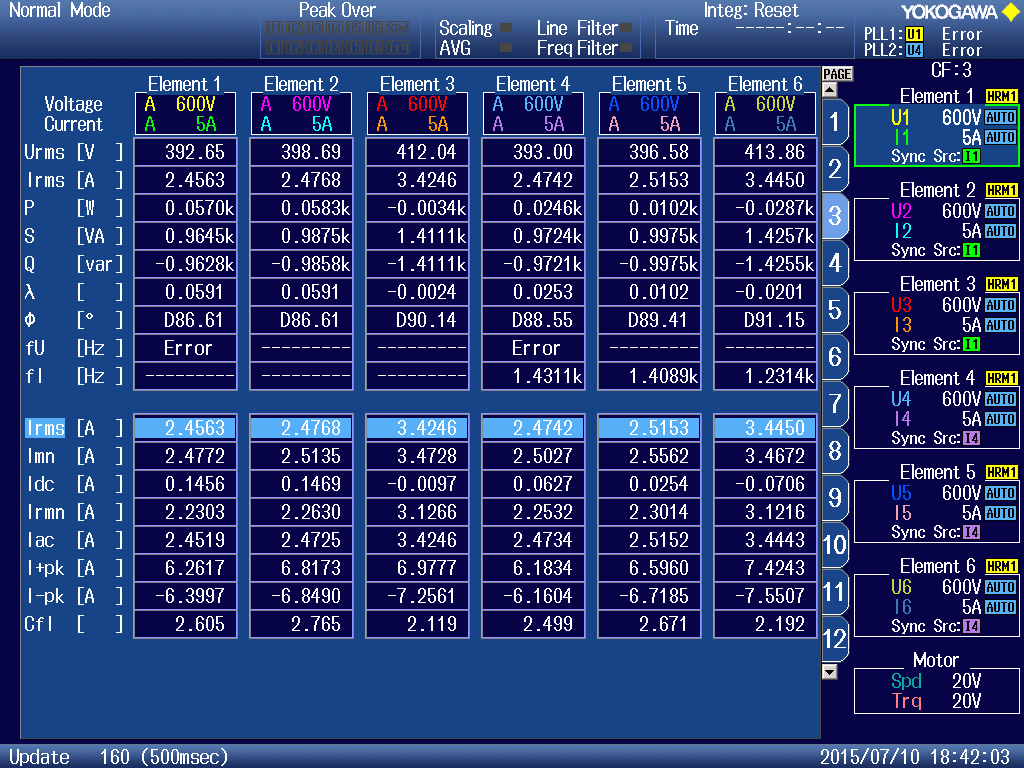
\includegraphics[width=1\linewidth]{aqs/0002}
		\caption{Tensões nos capacitores de barramento e correntes de saída dos inversores da fase B ($W_{b1}$, $W_{b2}$ e $W_{b3}$) e da fase A ($W_{a1}$, $W_{a2}$ e $W_{a3}$).}
		\label{fig:0002}
	\end{minipage}
	\quad
	\begin{minipage}[t]{0.45\textwidth} \centering
		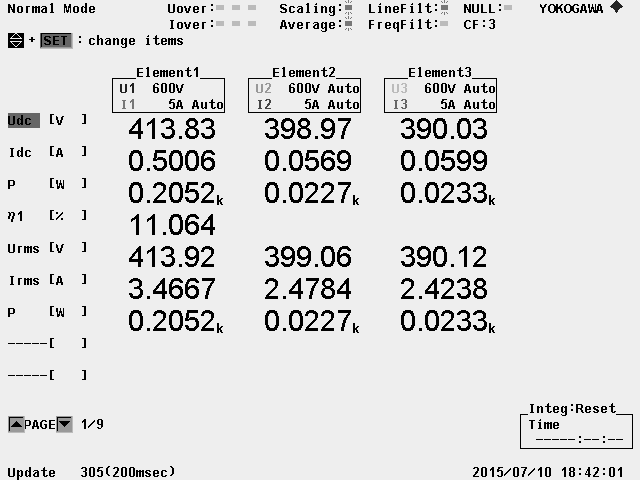
\includegraphics[width=1\linewidth]{aqs/TTZVSPWM0015}
		\caption{Tensões nos capacitores de barramento e correntes de saída dos inversores da fase C ($W_{c1}$, $W_{c2}$ e $W_{c3}$).}
		\label{fig:TTZVSPWM0015}
	\end{minipage}	
\end{figure}


\begin{figure}[!h]
	\centering
	\begin{minipage}[t]{0.45\textwidth}	\centering
		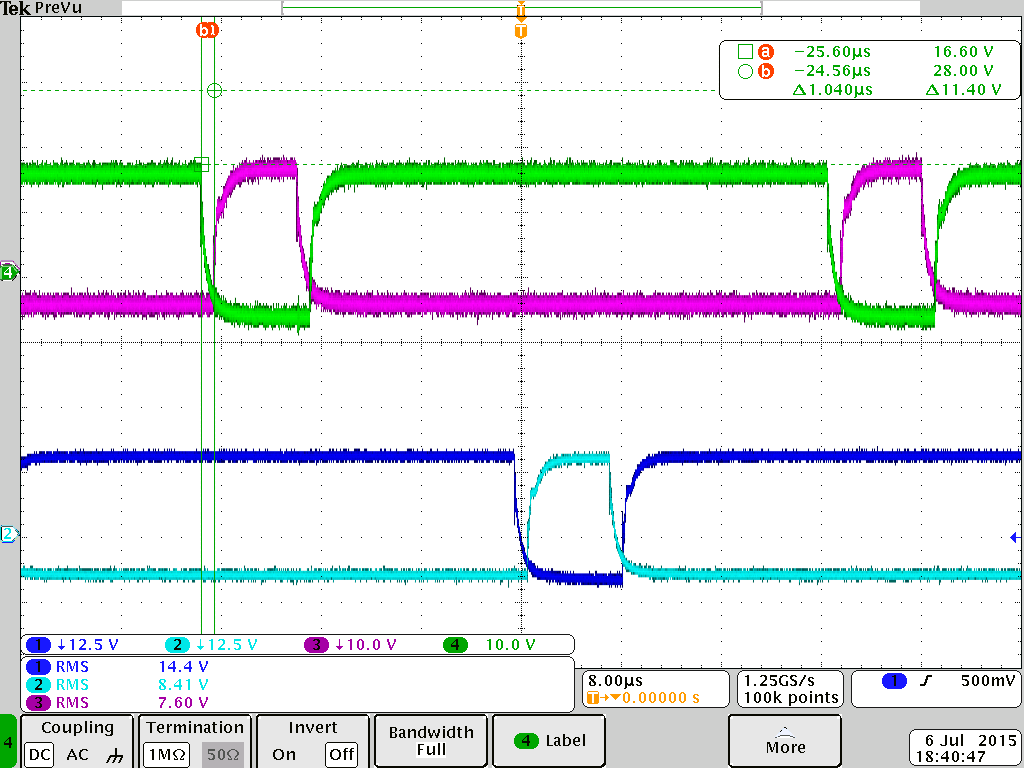
\includegraphics[width=1\linewidth]{aqs/tek0003}
		\caption{Tempo morto medido no braço 1 do inversor A3}
		\label{fig:tek0003}
	\end{minipage}
	\quad
	\begin{minipage}[t]{0.45\textwidth} 	\centering
		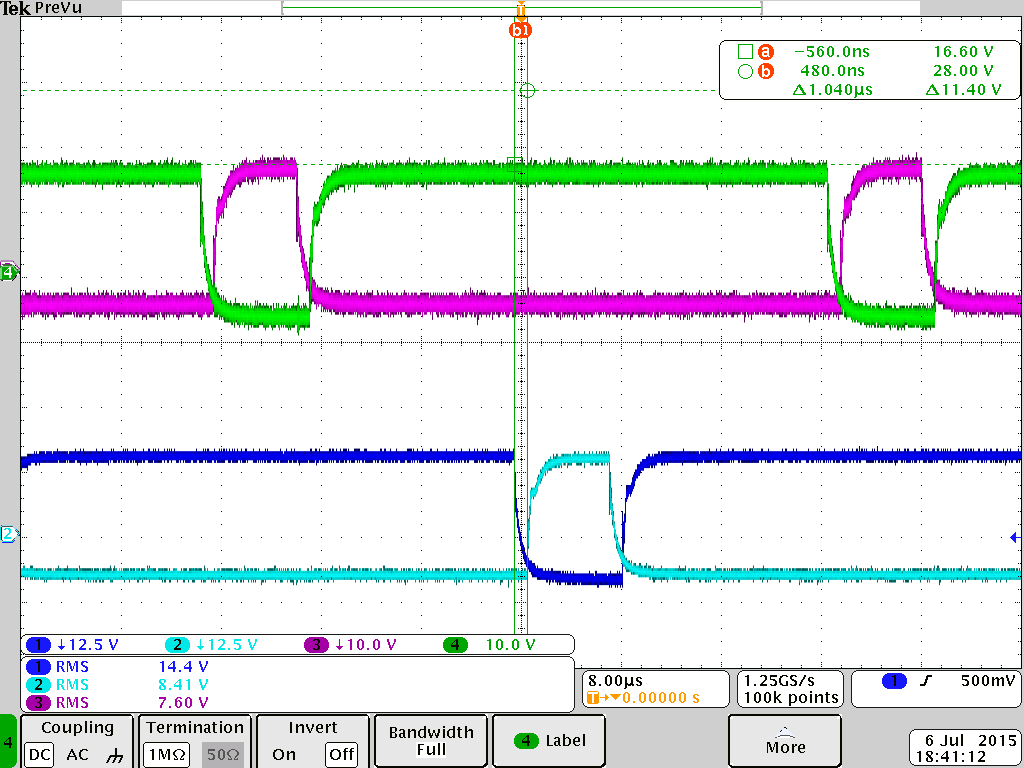
\includegraphics[width=1\linewidth]{aqs/tek0004}
		\caption{Tempo morto medido no braço 2 do inversor A3}
		\label{fig:tek0004}
	\end{minipage}	
\end{figure}


\begin{figure}[!h]
	\centering
	\begin{minipage}[t]{0.45\textwidth}	\centering
		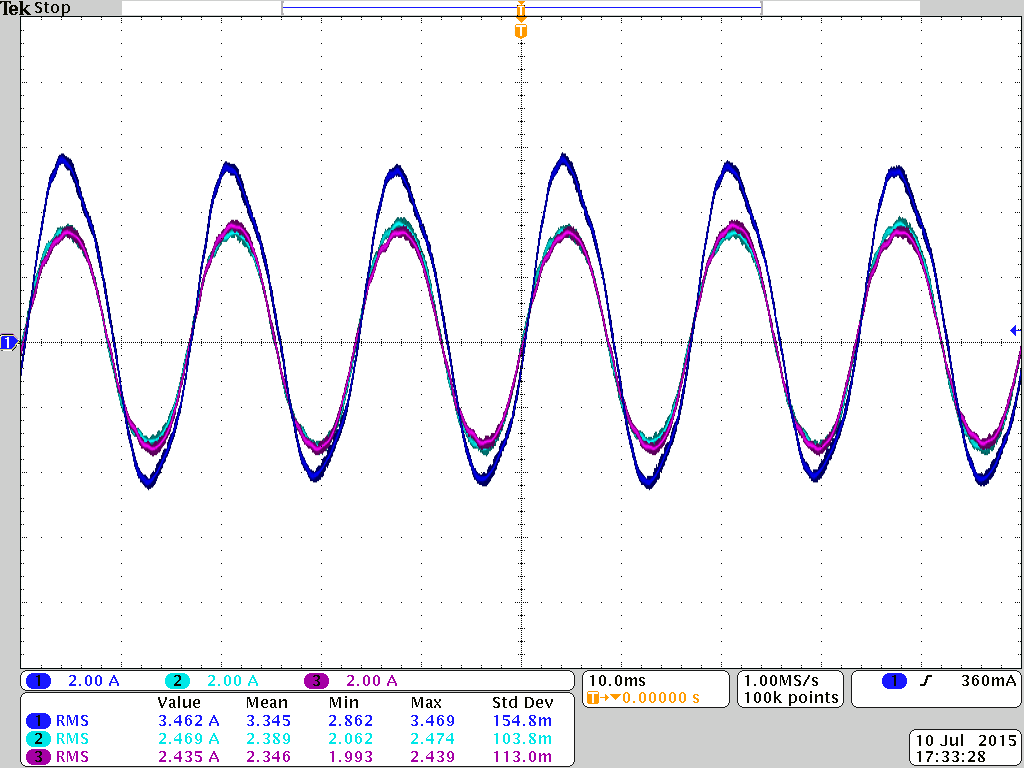
\includegraphics[width=1\linewidth]{aqs/tek0001}
		\caption{Correntes na fase C com um degrau de carga.}
		\label{fig:currenttek0001}
	\end{minipage}
	\quad
	\begin{minipage}[t]{0.45\textwidth} 	\centering
		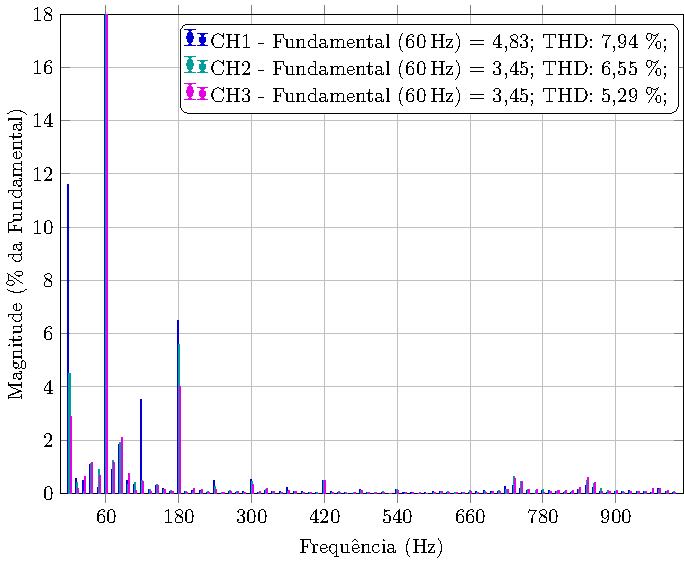
\includegraphics[width=1\linewidth]{aqs/tek0001FFT}
		\caption{Espectro das correntes na fase C com um degrau de carga.}
		\label{fig:currentFFTtek0001}
	\end{minipage}	
\end{figure}

\clearpage
\section{Axiomas ou postulados}

Na lógica tradicional, um axioma ou postulado é uma sentença ou proposição que não é provada ou demonstrada e é considerada como óbvia ou como um consenso inicial necessário para a construção ou aceitação de uma teoria. Por essa razão, é aceito como verdade e serve como ponto inicial para dedução e inferências de outras verdades (dependentes de teoria).


Na matemática, um axioma é uma hipótese inicial de qual outros enunciados são logicamente derivados. Pode ser uma sentença, uma proposição, um enunciado ou uma regra que permite a construção de um sistema formal. Diferentemente de teoremas, axiomas não podem ser derivados por princípios de dedução e nem são demonstráveis por derivações formais, simplesmente porque eles são hipóteses iniciais. Isto é, não há mais nada a partir do que eles seguem logicamente (em caso contrário eles seriam chamados teoremas). Em muitos contextos, "axioma", "postulado" e "hipótese" são usados como sinônimos.


\begin{axioma}[Axioma de Igualdade]
	Supondo $\mathfrak{L}$, uma linguagem de primeira ordem. para cada variável $x$, a fórmula $x = x$ é universalmente válida.
\end{axioma}


\begin{postulado}[Postulado de Igualdade]
	Supondo $\mathfrak{L}$, uma linguagem de primeira ordem. para cada variável $x$, a fórmula $x = x$ é universalmente válida.
\end{postulado}


\section{Teorema}


Na matemática, um teorema é uma afirmação que pode ser provada como verdadeira através de outras afirmações já demonstradas, como outros teoremas, juntamente com afirmações anteriormente aceitas, como axiomas. Prova é o processo de mostrar que um teorema está correto. O termo teorema foi introduzido por Euclides, em Elementos, para significar "afirmação que pode ser provada". Em grego, originalmente significava "espetáculo" ou "festa". Atualmente, é mais comum deixar o termo "teorema" apenas para certas afirmações que podem ser provadas e de grande "importância matemática", o que torna a definição um tanto subjetiva.

\begin{teorema}[Teorema de Pitágoras]
	Em qualquer triângulo retângulo, o quadrado do comprimento da hipotenusa é igual à soma dos quadrados dos comprimentos dos catetos. 
\end{teorema}


\subsection{Terminologia}



Usualmente deixa-se o termo ``teorema'' apenas para as afirmações que podem ser provadas de grande importância. Assim, são dados outros nomes para os outros tipos dessas afirmações:

\begin{description}
	\item[Proposição:] Uma Proposição é uma sentença não associada a algum outro teorema, de simples prova e de importância matemática menor.
	\item[Lema:] Um Lema é um "pré-teorema", um teorema que serve para ajudar na prova de outro teorema maior. A distinção entre teoremas e lemas é um tanto quanto arbitrária, uma vez que grandes resultados são usados para provar outros. Por exemplo, o Lema de Gauss e o Lema de Zorn são muito interessantes de per se, e muitos autores os denominam de Lemas, mesmo que não os usem para provar alguma outra coisa.
	\item[Corolário:] Um Corolário é uma consequência direta de outro teorema ou de uma definição, muitas vezes tendo suas demonstrações omitidas, por serem simples.
\end{description}


\begin{corolario}
	Em qualquer triângulo retângulo, a hipotenusa é maior que qualquer um dos catetos, mas menor que a soma deles.
\end{corolario}

Alguns outros termos também são usados, por mais que raros e com definição menos rigorosa, basicamente sendo usadas quando não se quer usar a a palavra "teorema":

Regra.
Lei, que também pode se referir a axiomas, regras de dedução e a distribuições de Probabilidade.
Princípio.
Algoritmo (como em Algoritmo da Divisão), muito raro e diferente do conceito com o mesmo nome que é um dos estudos centrais da Ciência da Computação.
Paradoxo, usado quando a afirmação vai aparentemente de encontro com alguma outra verdade ou com alguma noção intuitiva. Entretanto, tal termo também pode ser usado para afirmações falsas que aparentem ser verdadeiras em um primeiro momento.

Alguns teoremas continuam a ser chamados de Conjecturas logo após serem provados (por exemplo, a Conjectura de Poincaré). O termo conjectura é usado para afirmações que não se sabe se são verdadeiras, e que acredita-se que são verdadeiras, mas nunca ninguém conseguiu prová-las nem negá-las (às vezes conjecturas são chamadas de hipóteses (como em Hipótese de Riemann), obviamente, num sentido diferente do aqui já descrito).


\subsection{Conjectura ou hipótese}

Uma conjectura é uma ideia, fórmula ou frase, a qual não foi provada ser verdadeira, baseada em suposições ou ideias com fundamento não verificado. As conjecturas utilizadas como prova de resultados matemáticos recebem o nome de hipóteses.



\begin{conjectura}[Conjectura dos primos gêmeos]	
	Existem infinitos números primos gêmeos.
\end{conjectura}

Um par de primos é chamado de primos gêmeos se eles são dois números primos $p$, $q$ tais que $q = p + 2$.



\subsection{Lema}

Na Matemática, um lema é um teorema que é usado como um passo intermediário para atingir um resultado maior, provado em outro teorema. Normalmente o lema tem pouca serventia além de servir ao propósito do teorema que o utiliza, mas isto não é uma regra, e a classificação entre lemas e teoremas é arbitrária\footnote{Wikipédia}.


\begin{lema}	
	Given two line segments whose lengths are $a$ and $b$ respectively there is a 
	real number $r$ such that $b=ra$.
\end{lema}



Unnumbered theorem-like environments are also possible.

\begin{observacao}
	This statement is true, I guess.
\end{observacao}

And the next is a somewhat informal definition


\begin{definicao}[Fibration]
	A fibration is a mapping between two topological spaces that has the homotopy lifting property for every space $X$.
\end{definicao}

\begin{exemplo}[Fibration]
	A fibration is a mapping between two topological spaces that has the homotopy lifting property for every space $X$.
\end{exemplo}


\begin{exercicio}
	Este é um exercício
	
\end{exercicio}

\begin{exercicio}
	Mais um exercício para vocês...
	
\end{exercicio}


\begin{condicao}[Fibration]
	A fibration is a mapping between two topological spaces that has the homotopy lifting property for every space $X$.
\end{condicao}
Theorem styles

\begin{description}
	\item[definition] boldface title, romand body. Commonly used in definitions, conditions, problems and examples.
	\item[plain] boldface title, italicized body. Commonly used in theorems, lemmas, corollaries, propositions and conjectures.
	\item[remark] italicized title, romman body. Commonly used in remarks, notes, annotations, claims, cases, acknowledgments and conclusions. 
\end{description}



\subsection{Recuo do ambiente \texttt{citacao}}

Na produção de artigos (opção \texttt{article}), pode ser útil alterar o recuo
do ambiente \texttt{citacao}. Nesse caso, utilize o comando:

\begin{verbatim}
   \setlength{\ABNTEXcitacaorecuo}{1.8cm}
\end{verbatim}

Quando um documento é produzido com a opção \texttt{twocolumn}, a classe
\textsf{abntex2} automaticamente altera o recuo padrão de 4 cm, definido pela
ABNT NBR 10520:2002 seção 5.3, para 1.8 cm.


\section{Mais exemplos no Modelo Canônico de Trabalhos Acadêmicos}

Este modelo de artigo é limitado em número de exemplos de comandos, pois são
apresentados exclusivamente comandos diretamente relacionados com a produção de
artigos.

Para exemplos adicionais de \abnTeX\ e \LaTeX, como inclusão de figuras,
fórmulas matemáticas, citações, e outros, consulte o documento
\citeonline{abntex2modelo}.

\section{Consulte o manual da classe \textsf{abntex2}}

Consulte o manual da classe \textsf{abntex2} \cite{abntex2classe} para uma
referência completa das macros e ambientes disponíveis.

% ---
% Finaliza a parte no bookmark do PDF, para que se inicie o bookmark na raiz
% ---
\bookmarksetup{startatroot}% 
% ---

% ---
% Conclusão
% ---
\section*{Considerações finais}
\addcontentsline{toc}{section}{Considerações finais}

\lipsum[1]

\begin{citacao}
\lipsum[2]
\end{citacao}

\lipsum[3]

% ----------------------------------------------------------
% ELEMENTOS PÓS-TEXTUAIS
% ----------------------------------------------------------
\postextual


% ---
% Título e resumo em língua estrangeira
% ---

% \twocolumn[    		% INICIO DE ARTIGO EM DUAS COLUNAS



% ]  				% FIM DE ARTIGO EM DUAS COLUNAS
% ---

\newpage
\pagestyle{plain}
%
% ----------------------------------------------------------
% Referências bibliográficas
% ----------------------------------------------------------
\bibliography{abntex2-modelo-references}

% ----------------------------------------------------------
% Glossário
% ----------------------------------------------------------
%
% Há diversas soluções prontas para glossário em LaTeX. 
% Consulte o manual do abnTeX2 para obter sugestões.
%
%\glossary

% ----------------------------------------------------------
% Apêndices
% ----------------------------------------------------------

\newpage
\pagestyle{notasUFSC}
% ---
% Inicia os apêndices
% ---
\begin{apendicesenv}

% ---
\chapter{Relações Trigonométricas}
% ---

\section{Deslocamentos Angulares}
\subsection{Deslocamento de 90 graus}
\begin{eqnarray}
\sin(\theta + \tfrac{\pi}{2}) &= +\cos \theta \\
\cos(\theta + \tfrac{\pi}{2}) &= -\sin \theta \\
\tan(\theta + \tfrac{\pi}{2}) &= -\cot \theta \\
\csc(\theta + \tfrac{\pi}{2}) &= +\sec \theta \\
\sec(\theta + \tfrac{\pi}{2}) &= -\csc \theta \\
\cot(\theta + \tfrac{\pi}{2}) &= -\tan \theta
\end{eqnarray}

\subsection{Deslocamento de 180 graus}
\begin{eqnarray}
\sin(\theta + \pi) &= -\sin \theta \\
\cos(\theta + \pi) &= -\cos \theta \\
\tan(\theta + \pi) &= +\tan \theta \\
\csc(\theta + \pi) &= -\csc \theta \\
\sec(\theta + \pi) &= -\sec \theta \\
\cot(\theta + \pi) &= +\cot \theta 
\end{eqnarray}

\subsection{Deslocamento de 360 graus}
\begin{eqnarray}
\sin(\theta + 2\pi) &= +\sin \theta \\
\cos(\theta + 2\pi) &= +\cos \theta \\
\tan(\theta + 2\pi) &= +\tan \theta \\
\csc(\theta + 2\pi) &= +\csc \theta \\
\sec(\theta + 2\pi) &= +\sec \theta \\
\cot(\theta + 2\pi) &= +\cot \theta
\end{eqnarray}




\section{Relações de soma e subtração}

\begin{eqnarray}
\sin(\alpha \pm \beta) & =& \sin \alpha \cos \beta \pm \cos \alpha \sin \beta \\
\cos(\alpha \pm \beta) & =& \cos \alpha \cos \beta \mp \sin \alpha \sin \beta \\
\tan(\alpha \pm \beta) &= &\frac{\tan \alpha \pm \tan \beta}{1 \mp \tan \alpha \tan \beta}\\
\arcsin\alpha \pm \arcsin\beta &=& \arcsin\left(\alpha\sqrt{1-\beta^2} \pm \beta\sqrt{1-\alpha^2}\right)\\
\arccos\alpha \pm \arccos\beta &=& \arccos\left(\alpha\beta \mp \sqrt{(1-\alpha^2)(1-\beta^2)}\right)\\
\arctan\alpha \pm \arctan\beta &=&\arctan\left(\frac{\alpha \pm \beta}{1 \mp \alpha\beta}\right)
\end{eqnarray}



\section{Ângulo duplo}


\begin{eqnarray}
\sin 2\theta &=& 2 \sin \theta \cos \theta  = \frac{2 \tan \theta} {1 + \tan^2 \theta} \\
\cos 2\theta &=& \cos^2 \theta - \sin^2 \theta = 2 \cos^2 \theta - 1 = 1 - 2 \sin^2 \theta = \frac{1 - \tan^2 \theta} {1 + \tan^2 \theta}\\
\tan 2\theta &=& \frac{2 \tan \theta} {1 - \tan^2 \theta}\\
\cot 2\theta &=& \frac{\cot^2 \theta - 1}{2 \cot \theta}
\end{eqnarray}


\section{Ângulo Triplo}


\begin{eqnarray}
\sin 3\theta &=& - \sin^3\theta + 3 \cos^2\theta \sin\theta 
= - 4\sin^3\theta + 3\sin\theta  \\
\cos 3\theta  &=& \cos^3\theta - 3 \sin^2 \theta\cos \theta =
4 \cos^3\theta - 3 \cos\theta \\
\tan 3\theta &=& \frac{3 \tan\theta - \tan^3\theta}{1 - 3 \tan^2\theta}\\
\cot 3\theta &=& \frac{3 \cot\theta - \cot^3\theta}{1 - 3 \cot^2\theta}
\end{eqnarray}


\section{Meio ângulo}

\begin{eqnarray}
\sin \frac{\theta}{2} &=& \sgn \left(2 \pi - \theta + 4 \pi \left\lfloor \frac{\theta}{4\pi} \right\rfloor \right) \sqrt{\frac{1 \! - \! \cos \theta}{2}}\\
\sin^2\frac{\theta}{2} &=& \frac{1-\cos\theta}{2}\\
\cos \frac{\theta}{2} &=& \sgn \left(\pi + \theta + 4 \pi \left\lfloor \frac{\pi - \theta}{4\pi} \right\rfloor \right) \sqrt{\frac{1 + \cos\theta}{2}}\\
\cos^2\frac{\theta}{2} &=&\frac{1+\cos\theta}{2}\\
\tan \frac{\theta}{2} &=& \csc \theta - \cot \theta = \pm\, \sqrt{1 - \cos \theta \over 1 + \cos \theta} = \frac{\sin \theta}{1 + \cos \theta} = \frac{1-\cos \theta}{\sin \theta} \\
\tan\frac{\eta+\theta}{2} &=& \frac{\sin\eta+\sin\theta}{\cos\eta+\cos\theta} \\
\tan\left(\frac{\theta}{2} + \frac{\pi}{4}\right) &= &\sec\theta + \tan\theta \\
\sqrt{\frac{1 - \sin\theta}{1 + \sin\theta}}  &= &\frac{1 - \tan(\theta/2)}{1 + \tan(\theta/2)}\\
\tan\tfrac{1}{2}\theta  &=& \frac{\tan\theta}{1 + \sqrt{1+\tan^2\theta}} \left(-\tfrac{\pi}{2} < \theta < \tfrac{\pi}{2} \right)\\
\cot \frac{\theta}{2} & =& \csc \theta + \cot \theta = \pm\, \sqrt{1 + \cos \theta \over 1 - \cos \theta} = \frac{\sin \theta}{1 - \cos \theta} = \frac{1 + \cos \theta}{\sin \theta} 
\end{eqnarray}


\section{Redução de Potência}

\begin{eqnarray}
\sin^2\theta &=& \frac{1 - \cos 2\theta}{2}\\
\cos^2\theta &=& \frac{1 + \cos 2\theta}{8}\\
\sin^2\theta \cos^2\theta &=& \frac{1 - \cos 4\theta}{8}
\end{eqnarray}


\begin{eqnarray}
\sin^3\theta &=& \frac{3 \sin\theta - \sin 3\theta}{4}\\
\cos^3\theta &=& \frac{3 \cos\theta + \cos 3\theta}{4}\\
\sin^3\theta \cos^3\theta &=& \frac{3\sin 2\theta - \sin 6\theta}{32}
\end{eqnarray}



\section{Produto para soma}
\begin{eqnarray}
2\cos \theta \cos \varphi &=& {{\cos(\theta - \varphi) + \cos(\theta + \varphi)}}\\
2\sin \theta \sin \varphi &=& {{\cos(\theta - \varphi) - \cos(\theta + \varphi)} }\\
2\sin \theta \cos \varphi &=& {{\sin(\theta + \varphi) + \sin(\theta - \varphi)} }\\
2\cos \theta \sin \varphi &=& {{\sin(\theta + \varphi) - \sin(\theta - \varphi)} }\\
\tan \theta \tan \varphi &=&\frac{\cos(\theta-\varphi)-\cos(\theta+\varphi)}{\cos(\theta-\varphi)+\cos(\theta+\varphi)}
\end{eqnarray}


\section{Soma para Produto}
\begin{eqnarray}
\sin \theta \pm \sin \varphi &=& 2 \sin\left( \frac{\theta \pm \varphi}{2} \right) \cos\left( \frac{\theta \mp \varphi}{2} \right)\\
\cos \theta + \cos \varphi &=& 2 \cos\left( \frac{\theta + \varphi} {2} \right) \cos\left( \frac{\theta - \varphi}{2} \right)\\
\cos \theta - \cos \varphi &=& -2\sin\left( {\theta + \varphi \over 2}\right) \sin\left({\theta - \varphi \over 2}\right)\\
\end{eqnarray}



\end{apendicesenv}
% ---

\newpage
% ----------------------------------------------------------
% Anexos
% ----------------------------------------------------------
\cftinserthook{toc}{AAA}
% ---
% Inicia os anexos
% ---
%\anexos
\begin{anexosenv}

\chapter{Datasheet para o conjunto inversor monofásico SPCIM 450-60-20}

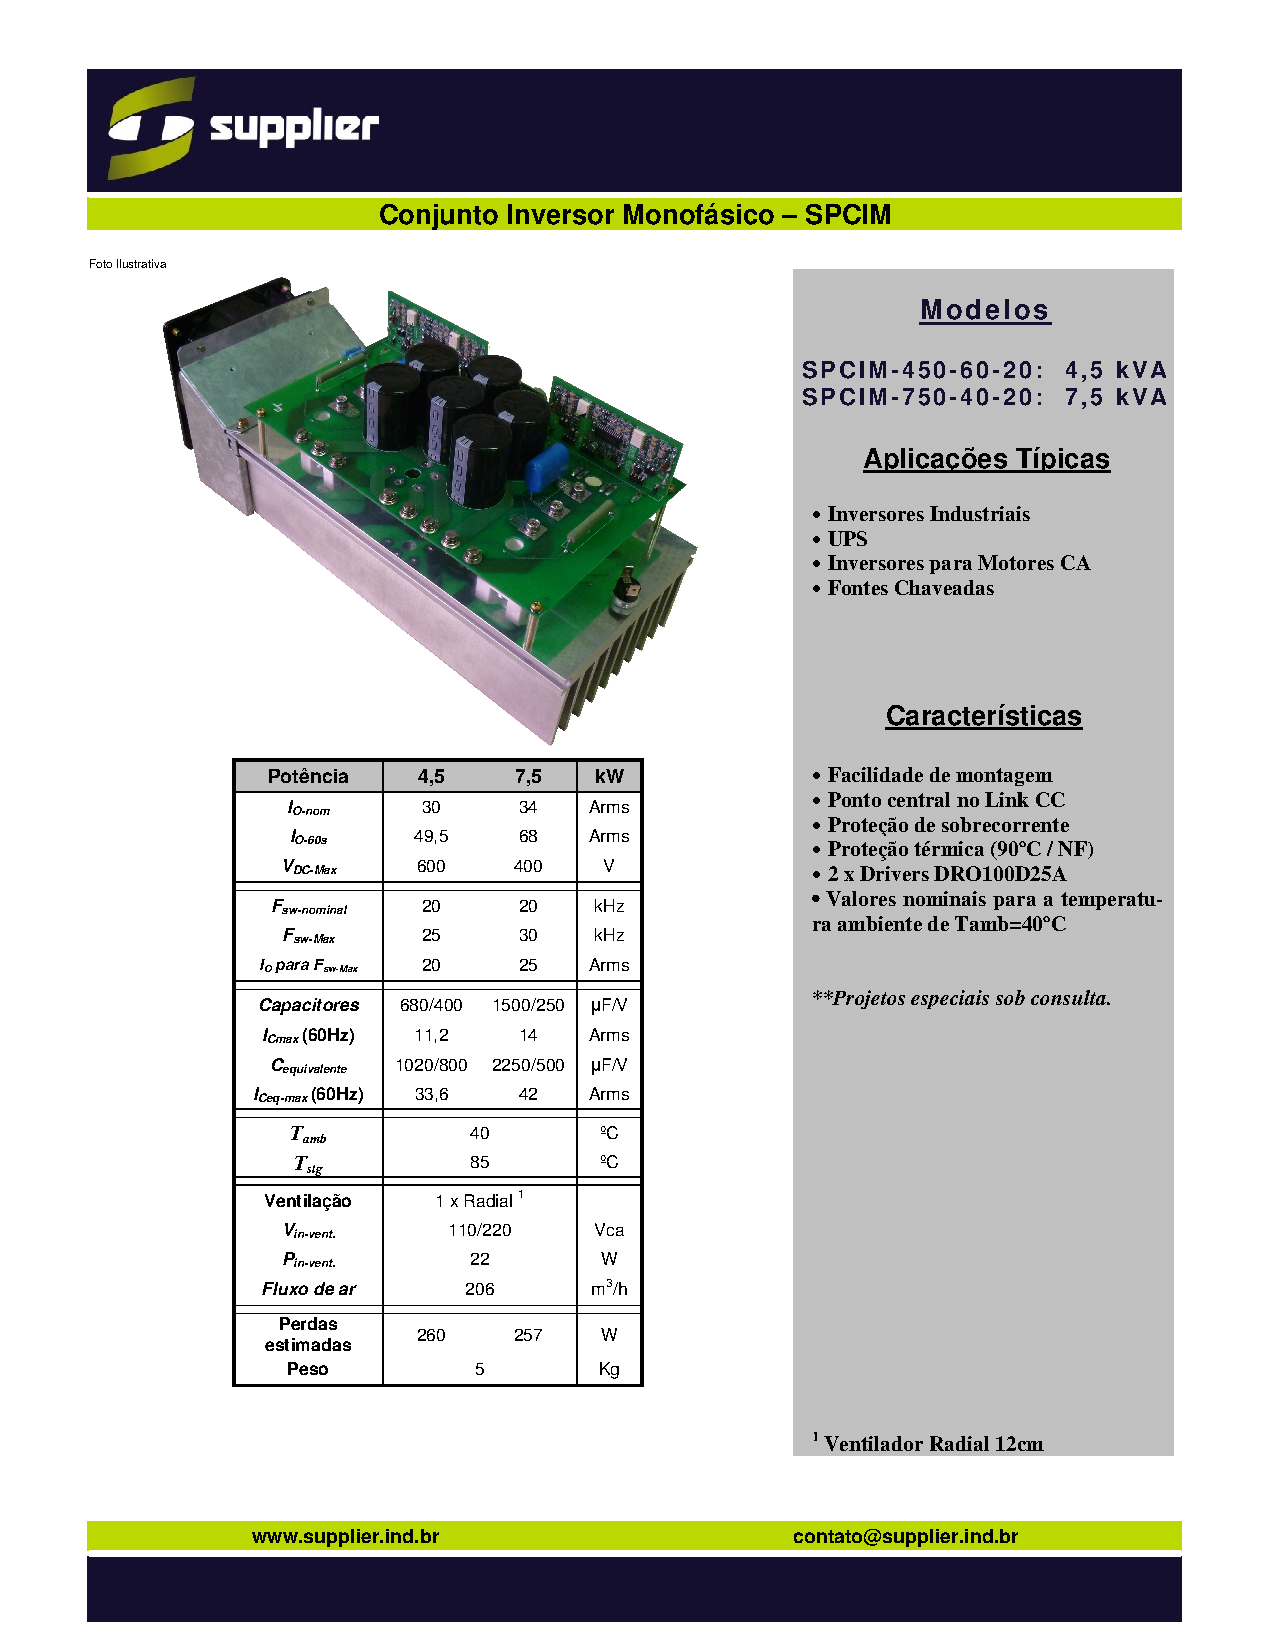
\includepdf[pages=-]{docs/SPCIM450-60-20.pdf}

\end{anexosenv}

\end{document}
